% !TeX root = ../../tfg.tex
% !TeX encoding = utf8
%
\section{Recurrencias continuas en varias variables}\label{ch:ideas_recurrencias_continuas_en_varias_variables}

\subsection{Idea}

Como hemos visto en la construcción de los polinomios de 
Bernstein \ref{ch:Bernstein}, para construir aproximaciones se necesitan puntos 
y cada punto nuevo a añadir añade complejidad al polinomio construido.

¿Es posible construir una función convergente de complejidad constante?

Combinando esta pregunta con el concepto de recurrencia discreta se me ocurrió definir 
la siguiente estructura. 

La dejo escrita simplemente porque me parece curiosa y quizás nos pueda ayudar en algún momento, 
no he buscado si alguien ha definido ya algo parecido con anterioridad, probablemente si es de utilidad sí. 

\subsection{Explicación}  

Comenzaré presentando la estructura con ejemplo:  

Supongamos que en el plano euclídeo se tiene definida una curva $\sigma_0$, 
que sin pérdida de generalidad restringe su dominio del intervalo $[0,1]$ al plano. 
Se define pues a la función recurrente continua de la curva $\sigma_0$, 
a la que denotaremos como $\mathcal S_{\sigma_0}$;
como la suma infinita numerable de
 las curvas $\sigma_n :[0,1] \longrightarrow \R^2$ con $n$ natural y construido de manera recursiva como
 $$\sigma_n(t) = \sigma_{n-1}(1) + \sigma_0(t) - \sigma_0(0)$$.  

 es decir $\mathcal S_{\sigma_0}(n + t) = \sigma_n(t)$  con $n$ natural y $t \in [0,1]$.

 Un ejemplo sencillo de esto sería el mostrado en la figura \ref{img:idea_recurrencia_ejemplo_sencillo}.  
 \begin{figure}[h!]
 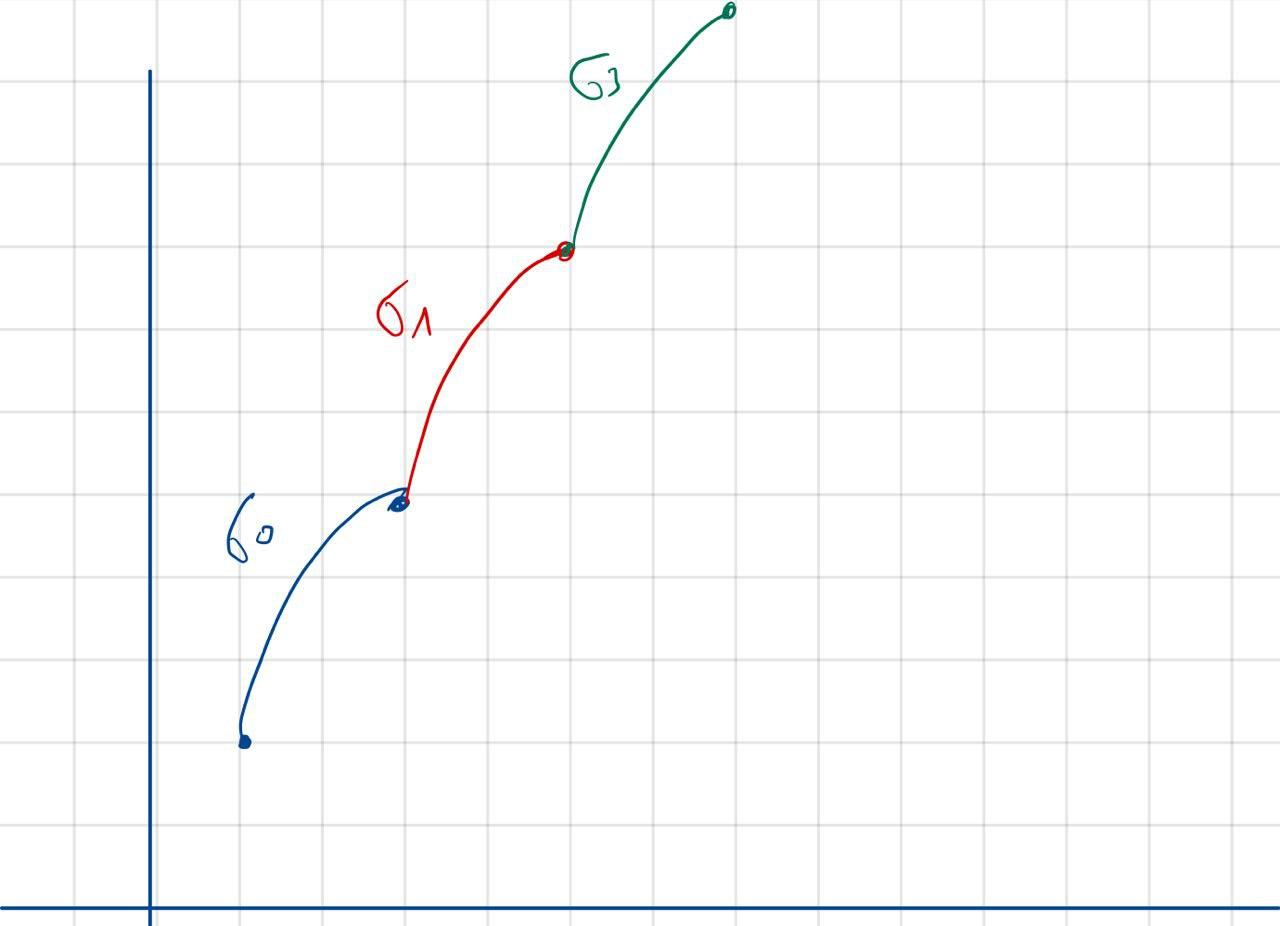
\includegraphics[width=\textwidth]{ideas/recurencias_continuas/ejemplo_sencillo.jpg}
 \caption{Ejemplo sencillo de como quería los tres primeros elementos de la sucesión de sigmas.}
 \label{img:idea_recurrencia_ejemplo_sencillo}
\end{figure}

Por cómo se ha definido es fácil generalizar la construcción para que la curva se encuentre en 
espacios de mayor dimensión. 

Quizás a priori pueda no parecer interesante esta estructura, pero introduzcamos 
de manera informal nuevas restricciones a nuestro problema: 

Dado un plano se quiere construir una función que pase por los \textit{puntos rojos} 
evitando los \textit{negros}
. Figura \ref{img:idea_recurrencia_plano}. 

\begin{figure}[h!]
    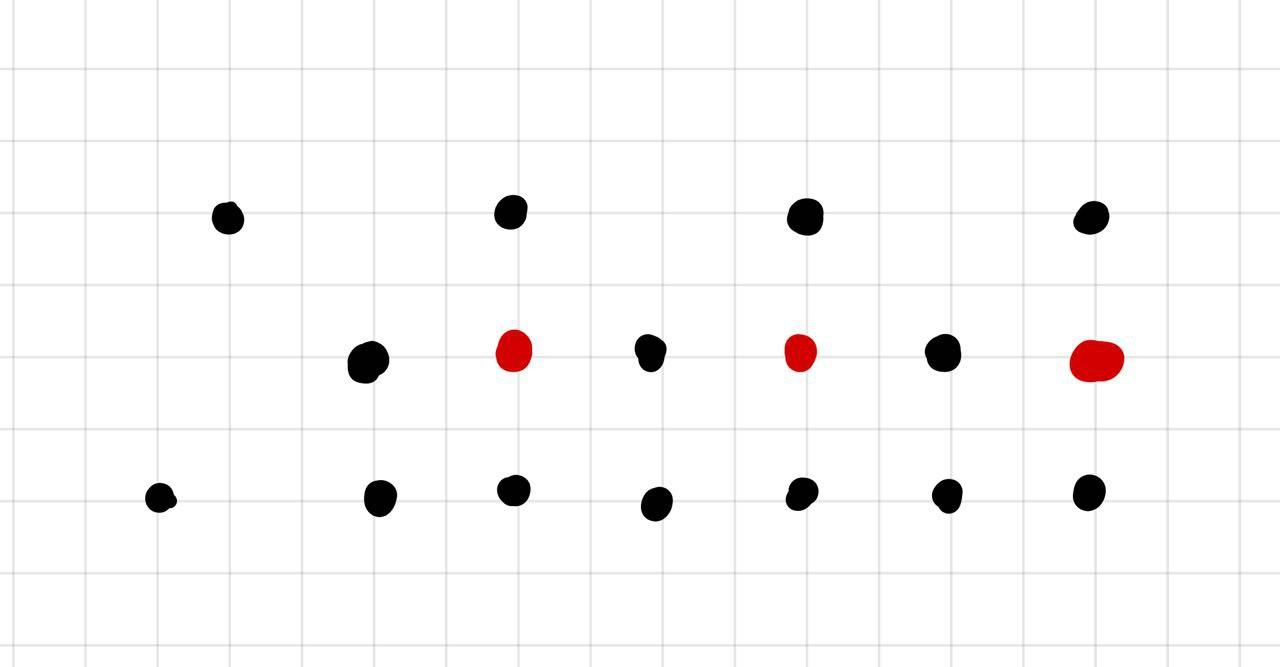
\includegraphics[width=\textwidth]{ideas/recurencias_continuas/ejemplo_de_plano.jpg}
    \caption{Plano del que evitar los puntos negros y tomar los rojos.}
    \label{img:idea_recurrencia_plano}
\end{figure}

Se podría resolver el problema valiéndose del polinomio de Bernstein o splines o
cualquier otro método, llegando a una función , como la dibujada en verde en la
figura \ref{img:idea_recurrencia_funcion_verde}

\begin{figure}[h!]
    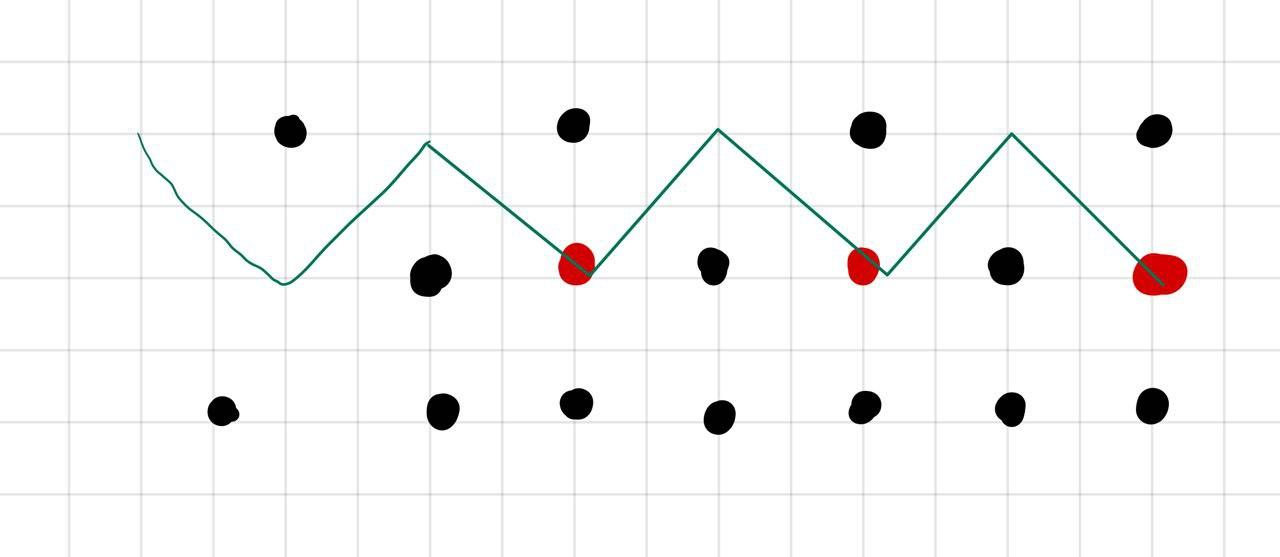
\includegraphics[width=\textwidth]{ideas/recurencias_continuas/funcion_continua.jpg}
    \caption{En verde ejemplo de función solución.}
    \label{img:idea_recurrencia_funcion_verde}
\end{figure} 

Sin embargo si hacemos uso de la estructura recién descrita, bastaría con 
calcular solo $\sigma_0$.
 Ver \ref{img:idea_recurrencia_sigma_cero}.  

\begin{figure}[h!]
    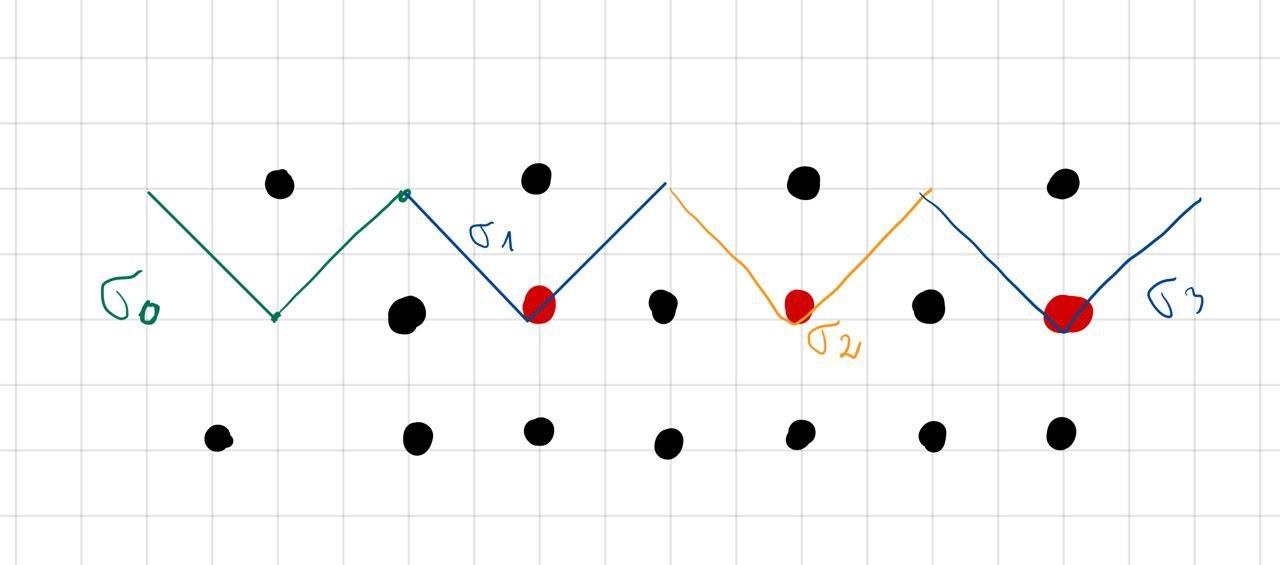
\includegraphics[width=\textwidth]{ideas/recurencias_continuas/recurrente.jpg}
    \caption{En verde ejemplo de función solución.}
    \label{img:idea_recurrencia_sigma_cero}
\end{figure} 


\subsection{ Preguntas que introduce esta estructura}

1. Nótese que ha sido necesaria cierta simetría o patrón en la estructura del ejemplo  

¿Se podría generalizar?   

De manera intuitiva las respuesta es sí. Bastaría con
\begin{enumerate}
 \item \textit{Dividir en la misma proporción el espacio} obteniendo las particiones $D_n$ (numeradas de izquierda a derecha).
 \item \textit{Superponer} las sucesivas $D_n$ de tal manera que obtenemos $\mathcal{D}$,
 \item Puesto que $\mathcal{D}$ contiene todos los puntos relevantes bastará con
 \item \textit{Trazar} en $D_0$ la curva $\sigma_0$ necesaria en  $\mathcal{D}$ y que 
  comience en un \textit{borde} cuya  posición relativa en $D_0$ sea 
  $\sigma_0(0)$, tal que el final de la curva trazada $\sigma_0(1)$, en la posición relativa 
  $D_1$  coincida con $\sigma_0(0)$. 
\end{enumerate}


Esta idea  de demostración intuitiva nos brinda las siguientes reflexiones 
sobre el modelo creado: 

\begin{itemize}
    \item En caso de que no haya hipótesis de patrón el costo computacional de construir 
    $\sigma_0$ es el mismo es el mismo (o mayor por las superposición) que el de construir la función entera. 

    \item Tiene la limitación de que el patrón se repite en una dimensión, ya que no deja de ser un grafo.
    (¿Fácilmente solventable  ampliando el número de $\sigma_0$?)
\end{itemize}

\subsection{Conclusiones}

Hasta el momento esta estructura aquí definida no deja de ser más de un delirio de curiosidad 
y no es fácilmente aplicable si no encontramos patrones en el espacio. 
Además se tiene la problemática de cómo se aplicaría esto al contexto
 minimizar mínimos cuadrados. 




